\section{Background}
\label{sec:background}




% \YJ{Merge this with the related work sections. Please add citations accordingly.}

%This section reviews graph representations, connectivity structures, and dynamic graph systems, and positions our work with respect to existing approaches.

% ============================================================
% \subsection{Graph Representation}
% ============================================================

\textbf{Static graph representation.}
High-performance graph processing systems rely on compressed
sparse formats such as CSR (Compressed Sparse Row) and CSC
(Compressed Sparse Column)~\cite{wheatman2018packed}.
These formats store adjacency information in contiguous arrays.
% ,enabling cache-efficient sequential access during traversal.
They form the foundation of major graph processing frameworks,
including Ligra~\cite{Shun2013Ligra},
Gunrock~\cite{Wang2016Gunrock}, and GraphIt~\cite{Zhang2018GraphIt}.
However, CSR and CSC are not suitable for dynamic workloads as vertex/edge insertions/deletions require rebuilding contiguous arrays, introducing significant overhead.
% under frequent updates.

\textbf{Dynamic graph representation.}
\begin{maybecut}
To support evolving graphs, recent systems propose specialized
in-memory structures that balance update cost and query
efficiency.
Terrace~\cite{pandey2021terrace} targets skewed graphs and uses
a hierarchical adjacency representation that adapts its storage
to vertex degree, improving locality and update efficiency on
power-law graphs~\cite{barabasi1999emergence}.
Spruce~\cite{shi2024spruce} combines compact indexing with
update-friendly adjacency organization, integrating dynamic
buffers with CSR-like sorted blocks and a read-optimized
concurrency protocol.
Aspen~\cite{dhulipala2019low} represents graphs using
compressed purely functional trees and exposes immutable
snapshot views that support concurrent readers across updates.
% CUT CANDIDATE: same one-line descriptions of Terrace/Spruce/Aspen
% repeated almost verbatim in experiment.tex's Baseline paragraph;
% condensed in \texttt{fixed} below.
\end{maybecut}
\begin{fixed}
To support evolving graphs, recent systems propose specialized
in-memory structures that balance update cost and query efficiency,
including Terrace~\cite{pandey2021terrace}, Spruce~\cite{shi2024spruce},
and Aspen~\cite{dhulipala2019low}; Section~\ref{sec:experiment} describes
each in detail as an experimental baseline.
\end{fixed}

\textbf{Incremental graph computation.}
A complementary approach maintains algorithm-specific state to avoid full recomputation after updates.
GraphBolt~\cite{mariappan2019graphbolt} tracks per-vertex aggregation dependencies across bulk-synchronous parallel (BSP) iterations and re-propagates only the delta induced by each mutation, supporting algorithms including SSSP and BFS.
DZiG~\cite{mariappan2021dzig} extends GraphBolt with sparsity-aware processing that skips zero-contribution edges, further reducing propagation work on sparse updates.
Both systems rely on Ligra-style static computation for initial results and are tightly coupled to the algorithm being executed; switching the query or source vertex requires rebuilding their cached state.


\begin{figure}[t]
    \centering
    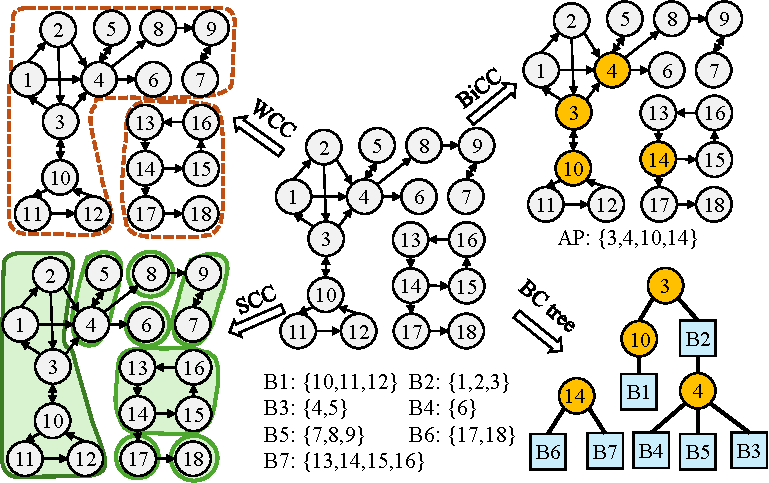
\includegraphics[width=\linewidth]{figures/scc_wcc_bcc-crop.pdf}
    \caption{Examples of weakly connected component (WCC), strongly connected component (SCC), biconnected component (BiCC), and block-cut (BC) tree.}
    \Description{An example directed graph annotated with its weakly connected components, strongly connected components, biconnected components, and the resulting block-cut tree.}
    % \YJ{TODO}}
    % \YJ{BC tree should look more like a "tree".\CQ{Done}}
    % }
    \label{fig:connectivity_example}
\end{figure}


% \YJ{Below discussions are too shallow. We need to touch the SOTA. Please rewrite.}
% \YJ{For static graphs, we should discuss adjacency matrix, adjacency list, and then emphasize CSR/CSC.}
% \YJ{For dynamic graphs, we need to clearly discuss the related works we have studied, such as, Terrace, Aspen, etc.}

% \textbf{Static graph representations.}
% Graph systems traditionally rely on several canonical representations.
% The earliest representations include adjacency matrices and adjacency lists.
% An adjacency matrix supports constant-time edge-existence queries but requires $O(n^2)$ memory, which makes it impractical for large sparse graphs.
% Adjacency lists significantly reduce memory usage to $O(n+m)$ and therefore form the basis of most traversal-based algorithms.

% Modern high-performance graph processing frameworks further adopt compressed sparse formats such as CSR (Compressed Sparse Row) and CSC (Compressed Sparse Column) ~\cite{wheatman2018packed}.
% These representations store adjacency information in contiguous arrays, enabling efficient sequential memory access and improved cache locality during neighborhood traversal.
% Consequently, CSR/CSC serve as the foundation of many static graph-processing systems, including Ligra~\cite{Shun2013Ligra}, Gunrock~\cite{Wang2016Gunrock}, and GraphIt~\cite{Zhang2018GraphIt}.

% Beyond classical CSR-based formats, some systems introduce alternative representations that support large-scale parallel graph analytics.
% For example, Aspen~\cite{dhulipala2019low} represents graphs using compressed purely-functional trees and exposes immutable \emph{snapshot} views for graph analytics.
% Each update produces a new graph version, enabling concurrent readers to operate on consistent snapshots while preserving structural sharing across versions.
% Although Aspen supports dynamic updates through versioning, its design primarily targets efficient analytics on static snapshots rather than fine-grained maintenance of continuously evolving graphs.

% Despite their efficiency for static workloads, CSR-based or snapshot-based representations are not well suited for highly dynamic environments.
% Edge insertions and deletions often require rebuilding large contiguous arrays or generating new graph versions, which introduces significant overhead when updates occur frequently.

% \textbf{Dynamic graph storage.}
% To support evolving graphs with interleaved updates and queries, recent systems propose specialized in-memory data structures that balance update cost, query efficiency, and memory usage.

% Terrace~\cite{pandey2021terrace} targets skewed streaming graphs and introduces a hierarchical adjacency representation in which a vertex’s neighbors are stored using different data structures depending on its degree.
% As vertex degrees evolve, the system dynamically reorganizes storage to improve locality and update efficiency on power-law graphs.

% Spruce~\cite{shi2024spruce} proposes a dynamic graph storage structure that combines compact indexing with update-friendly adjacency organization.
% It integrates dynamic buffers with CSR-like sorted blocks and introduces a read-optimized concurrency protocol that supports efficient simultaneous read and write operations.

%These systems primarily focus on efficiently storing and updating adjacency information.
%In contrast, our work focuses on maintaining reusable \emph{structural invariants} that directly accelerate downstream analytics.
%Rather than optimizing only the storage of edges, our approach maintains higher-level connectivity structures that reduce recomputation costs for traversal-based algorithms after graph updates.

% ============================================================
% \subsection{Graph Connectivity Structures}
% ============================================================

% \YJ{The below discussion is disorganized. In this section, the key is to explain "what is the algorithm (WCC, SCC)", not "how are they computed".}

% \YJ{Add references to each algorithm}

\textbf{Graph connectivity}
provides fundamental abstractions for graph topologies.
% As illustrated in Figure~\ref{fig:connectivity_example}, they capture structural relationships at multiple levels of granularity.
\textit{Weakly connected component (WCC)}
% In directed graphs, weakly connected components are 
is obtained by ignoring edge directions and grouping vertices that are reachable through undirected paths~\cite{vishkin1982log}.
WCCs partition the graph into independent regions that remain disconnected even when edge directions are ignored.
For the example in Figure~\ref{fig:connectivity_example}, the subgraph containing vertices $\{1\text{--}12\}$ forms one WCC, while vertices $\{13\text{--}18\}$ form another.
WCCs therefore represent the coarsest structural partition of the graph.

\textit{Strongly connected component (SCC)} 
% captures directed cyclic structure.
% An SCC 
is defined as a maximal subset of vertices such that every pair of vertices is mutually reachable~\cite{sharir1981strong}.
For the example in Figure~\ref{fig:connectivity_example}, vertices $\{1\text{--}3,10\text{--}12\}$, $\{13\text{--}16\}$ form a large SCC (shaded in green), while vertices $\{4,5\}$ and $\{7,9\}$ form small SCCs.

\textit{Biconnected component (BiCC)}
denotes a maximal subgraph that remains connected after removing any single vertex~\cite{westbrook1992maintaining}.
Vertices whose removal disconnects the graph are called articulation points (APs)~\cite{hopcroft1973algorithm}.
% Even within an SCC, strong connectivity does not necessarily imply structural robustness.
% To expose articulation structure, we temporarily treat edges as undirected and compute biconnected components (BiCCs).
% A BiCC is a maximal subgraph that remains connected after removing any single vertex. 
For the example in Figure~\ref{fig:connectivity_example},  $\{3,4,10,14\}$ are identified as APs.
The BiCC decomposition yields 7 blocks, including $B_1$ till $B_7$.
% such as 
% $b_1=\{10,11,12\}$,
% $b_2=\{1,2,3\}$,
% $b_3=\{4,5\}$,
% $b_4=\{6\}$, 
% $b_5=\{7,8,9\}$, 
% $b_6=\{17,18\}$, and
% $b_7=\{13,14,15,16\}$.

\textit{Block-cut (BC) tree} organizes the 
blocks and APs into a tree structure.
% are organized into a BC tree, which is always a tree even though the original graph may contain cycles.
For example, AP vertex 10 connects blocks $B_2$ and $B_1$, while AP vertex 14 connects blocks $B_6$ and $B_7$.
This tree structure explicitly exposes articulation boundaries within strongly connected regions.
% These connectivity abstractions are algorithm-independent structural invariants.
% They expose natural boundaries and hierarchical structure that many traversal-based algorithms implicitly rediscover during execution.

% \YJ{Might need an example figure to explain WCC, SCC, and BC tree.}
% \YJ{Can we use Figure 1?}



% ============================================================
%\subsection{Dynamic Graph Algorithms}
% ============================================================

%Fully dynamic graph algorithms maintain connectivity, reachability, or shortest paths under edge insertions and deletions.
%Early work studied dynamic transitive closure and APSP~\cite{King1999TransitiveClosure,Demetrescu2004DynamicAPSP}.
%Incremental approaches address SSSP and centrality updates~\cite{Ramalingam1996Incremental,Nasre2014IncBC}.

%Recent GPU-oriented research explores SCC and traversal acceleration, including frameworks such as ISPAN that combine synchronization strategies to accelerate SCC detection.

%\YJ{Should mention less here. Details should be in Related Work.}

%While these works improve specific dynamic problems, most are algorithm-specific and do not provide a reusable structural backbone for multiple downstream analytics.
%Our approach instead constructs a query-agnostic representation shared across algorithms.


